% Version 3 December 2023
% See section 11 of the User Manual for version history
%
%%%%%%%%%%%%%%%%%%%%%%%%%%%%%%%%%%%%%%%%%%%%%%%%%%%%%%%%%%%%%%%%%%%%%%
%%                                                                 %%
%% Please do not use \input{...} to include other tex files.       %%
%% Submit your LaTeX manuscript as one .tex document.              %%
%%                                                                 %%
%% All additional figures and files should be attached             %%
%% separately and not embedded in the \TeX\ document itself.       %%
%%                                                                 %%
%%%%%%%%%%%%%%%%%%%%%%%%%%%%%%%%%%%%%%%%%%%%%%%%%%%%%%%%%%%%%%%%%%%%%

%%\documentclass[referee,sn-basic]{sn-jnl}% referee option is meant for double line spacing

%%=======================================================%%
%% to print line numbers in the margin use lineno option %%
%%=======================================================%%

%%\documentclass[lineno,sn-basic]{sn-jnl}% Basic Springer Nature Reference Style/Chemistry Reference Style

%%======================================================%%
%% to compile with pdflatex/xelatex use pdflatex option %%
%%======================================================%%

%%\documentclass[pdflatex,sn-basic]{sn-jnl}% Basic Springer Nature Reference Style/Chemistry Reference Style

%%Note: the following reference styles support Namedate and Numbered referencing. By default the style follows the most common style. To switch between the options you can add or remove “Numbered” in the optional parenthesis.\\

%%The option is available for: sn-basic.bst, sn-vancouver.bst, sn-chicago.bst%

%%\documentclass[pdflatex,sn-nature]{sn-jnl}% Style for submissions to Nature Portfolio journals
%%\documentclass[pdflatex,sn-basic]{sn-jnl}% Basic Springer Nature Reference Style/Chemistry Reference Style
\documentclass[pdflatex, sn-mathphys-num, lineno]{sn-jnl}% Math and Physical Sciences Numbered Reference Style
%%\documentclass[pdflatex,sn-mathphys-ay]{sn-jnl}% Math and Physical Sciences Author Year Reference Style
%%\documentclass[pdflatex,sn-aps]{sn-jnl}% American Physical Society (APS) Reference Style
%%\documentclass[pdflatex,sn-vancouver,Numbered]{sn-jnl}% Vancouver Reference Style
%%\documentclass[pdflatex,sn-apa]{sn-jnl}% APA Reference Style
%%\documentclass[pdflatex,sn-chicago]{sn-jnl}% Chicago-based Humanities Reference Style

%%%% Standard Packages
%% additional latex packages if required can be included here>
\usepackage{graphicx}%
\usepackage{multirow}%
\usepackage{amsmath,amssymb,amsfonts}%
\usepackage{amsthm}%
\usepackage{mathrsfs}%
\usepackage[title]{appendix}%
\usepackage{xcolor}%
\usepackage{textcomp}%
\usepackage{manyfoot}%
\usepackage{booktabs}%
\usepackage{algorithm}%
\usepackage{algorithmicx}%
\usepackage{algpseudocode}%
\usepackage{listings}%

\usepackage{xspace}
\usepackage{standalone}

%% my package start

% for collabration and will remove before submit
\newcommand{\yy}[1]{\textcolor{cyan}{\textbf{[Yangyang: #1]}}}
\newcommand{\rd}[1]{\textcolor{green}{\textbf{[Dr.Yang: #1]}}}
\newcommand{\ty}[1]{\textcolor{orange}{\textbf{[Tingyou: #1]}}}
\newcommand{\qx}[1]{\textcolor{purple}{\textbf{[Qingxiang: #1]}}}

% for collabration and will remove before submit

\usepackage[detect-all=true]{siunitx}
\sisetup{
    scientific-notation=false,
    round-mode = places,
    round-precision = 2
}

\usepackage[acronym, automake, style=index, shortcuts]{glossaries-extra}

\setabbreviationstyle[acronym]{long-short}

% define glossaries
\makeglossaries
\newacronym{blat}{BLAT}{BLAST-like alignment tool}
\newacronym{llm}{LLM}{Large Language Model}
\newacronym{hmm}{HMM}{Hidden Markov Model}
\newacronym{gpu}{GPU}{Graphics Processing Unit}
\newacronym{hpc}{HPC}{High Performance Computing}
\newacronym{bert}{BERT}{Bidirectional Encoder Representations from Transformers}
\newacronym{gpt}{GPT}{Generative Pre-trained Transformer}

\newacronym{ide}{IDE}{Integrated Development Environment}
\newacronym{cd}{CD}{Continuous Development}
\newacronym{ucsc}{UCSC}{UCSC Genome Browser}
\newacronym{glm}{GLM}{Genomic Language Model}
\newacronym{lcglm}{LCGLM}{Long-Context Genomic Language Model}
\newacronym{snp}{SNP}{Single Nucleotide Polymorphism}
\newacronym{fm}{FM}{Foundational Model}
\newacronym{nlp}{NLP}{Natural Language Processing}

\newacronym{drs}{DRS}{direct RNA sequencing}
\newacronym{ont}{ONT}{Oxford Nanopore Technologies}
\newacronym{pb}{PacBio}{Pacific Biosciences}

\newacronym{go}{GO}{Gene Ontology}
\newacronym{r2c2}{R2C2}{Rolling Circle Amplification to Concatemeric Consensus}
\newacronym{pcr}{PCR}{Polymerase Chain Reaction}

\newacronym{tp}{TP}{True Positive}
\newacronym{fp}{FP}{False Positive}
\newacronym{fn}{FN}{False Negative}

\newcommand{\figref}[2]{Fig.~\hyperref[#1]{\ref*{#1}#2}}
\newcommand{\edfigref}[2]{Extended Data Fig.~\hyperref[#1]{\ref*{#1}#2}}
\newcommand{\edfigrefrg}[3]{Extended Data Fig.~\hyperref[#1]{\ref*{#1}#2-\ref*{#1}#3}}
%% my package end


%%%%%=============================================================================%%%%
%%%%  Remarks: This template is provided to aid authors with the preparation
%%%%  of original research articles intended for submission to journals published
%%%%  by Springer Nature. The guidance has been prepared in partnership with
%%%%  production teams to conform to Springer Nature technical requirements.
%%%%  Editorial and presentation requirements differ among journal portfolios and
%%%%  research disciplines. You may find sections in this template are irrelevant
%%%%  to your work and are empowered to omit any such section if allowed by the
%%%%  journal you intend to submit to. The submission guidelines and policies
%%%%  of the journal take precedence. A detailed User Manual is available in the
%%%%  template package for technical guidance.
%%%%%=============================================================================%%%%

%% as per the requirement new theorem styles can be included as shown below
\theoremstyle{thmstyleone}%
\newtheorem{theorem}{Theorem}%  meant for continuous numbers
%%\newtheorem{theorem}{Theorem}[section]% meant for sectionwise numbers
%% optional argument [theorem] produces theorem numbering sequence instead of independent numbers for Proposition
\newtheorem{proposition}[theorem]{Proposition}%
%%\newtheorem{proposition}{Proposition}% to get separate numbers for theorem and proposition etc.

\theoremstyle{thmstyletwo}%
\newtheorem{example}{Example}%
\newtheorem{remark}{Remark}%

\theoremstyle{thmstylethree}%
\newtheorem{definition}{Definition}%

\raggedbottom
\unnumbered% uncomment this for unnumbered level heads

\begin{document}

\title[Article Title]{Language model identify artificial chimeric read in Nanopore direct RNA sequencing data.}

%%=============================================================%%
%% GivenName	-> \fnm{Joergen W.}
%% Particle	-> \spfx{van der} -> surname prefix
%% FamilyName	-> \sur{Ploeg}
%% Suffix	-> \sfx{IV}
%% \author*[1,2]{\fnm{Joergen W.} \spfx{van der} \sur{Ploeg}
%%  \sfx{IV}}\email{iauthor@gmail.com}
%%=============================================================%%

\author[1]{\fnm{Yangyang} \sur{Li}}\email{yangyang.li@northwestern.edu}
\equalcont{These authors contributed equally to this work.}

% \author*[1,2]{\fnm{First} \sur{Author}}\email{iauthor@gmail.com}
\author[1]{\fnm{Tingyou} \sur{Wang}}\email{tingyou.wang@northwestern.edu}
\equalcont{These authors contributed equally to this work.}

\author[1]{\fnm{Qingxiang} \sur{Guo}}\email{qingxiang.guo@northwestern.edu}
\author*[1,2]{\fnm{Rendong} \sur{Yang}}\email{rendong.yang@northwestern.edu}

\affil[1]{\orgdiv{Department of Urology}, \orgname{Northwestern University Feinberg School of Medicine}, \orgaddress{\street{303 E Superior St}, \city{Chicago}, \postcode{60611}, \state{IL}, \country{USA}}}
\affil[2]{\orgdiv{Robert H. Lurie Comprehensive Cancer Center}, \orgname{Northwestern University Feinberg School of Medicine}, \orgaddress{\street{675 N St Clair St}, \city{Chicago}, \postcode{60611}, \state{IL}, \country{USA}}}

% \author[1,2]{\fnm{Third} \sur{Author}}\email{iiiauthor@gmail.com}
% \equalcont{These authors contributed equally to this work.}

% \affil*[1]{\orgdiv{Department}, \orgname{Organization}, \orgaddress{\street{Street}, \city{City}, \postcode{100190}, \state{State}, \country{Country}}}
% \affil[2]{\orgdiv{Department}, \orgname{Organization}, \orgaddress{\street{Street}, \city{City}, \postcode{10587}, \state{State}, \country{Country}}}
% \affil[3]{\orgdiv{Department}, \orgname{Organization}, \orgaddress{\street{Street}, \city{City}, \postcode{610101}, \state{State}, \country{Country}}}

%%==================================%%
%% Sample for unstructured abstract %%
%%==================================%%

\abstract{
    The accurate identification of chimeric reads is critical for ensuring the reliability of nanopore \gls{drs} data, which has emerged as a powerful tool for sequencing full-length RNA molecules while preserving native RNA modifications. Despite its potential, nanopore \gls{drs} is susceptible to the generation of chimeric reads, where fragments of distinct RNA molecules are incorrectly joined together, complicating downstream analyses such as transcriptome assembly and gene fusion detection.

    In this study, we present DeepChopper, a genomics language model specifically designed to detect and filter chimeric reads. Leveraging advanced long-range attention mechanisms and tailored tokenization strategies, DeepChopper effectively distinguishes true biological sequences from artificial constructs with high precision. We validated the performance of DeepChopper across multiple datasets, including \gls{ont} \gls{pcr} cDNA, \gls{ont} CapTrap-seq, \gls{ont} \gls{r2c2}, \gls{pb} cDNA, and \gls{pb} CapTrap-seq.

    Our results demonstrate that DeepChopper significantly outperforms existing methods, achieving up to a 94\% reduction in unsupported reads and consistently maintaining high support rates across diverse sequencing platforms. Additionally, DeepChopper effectively identified low-quality artificial sequences based on base quality scores and \gls{blat} identity, further enhancing the accuracy of nanopore \gls{drs} data.

    This study highlights the potential of DeepChopper to improve the integrity of nanopore \gls{drs} data, paving the way for more reliable genomic analyses and broadening the applicability of genomics language models in bioinformatics.}

\maketitle
\section{Main}\label{sec1}

% Outline
% 1. Sequencing history
% 2. Genomics LLM history
% 3. Challenges of LLM / efficiency of transformer and improvements (hyena)
% 3.1 long range
% 3.2 single nucleotide resolution
% 4. Cons of drs
% 5. Our method
% 6. Results
% 7. Conclusion

The advent of high-throughput sequencing technologies has revolutionized genomics, providing unprecedented insights into the genetic underpinnings of biological processes.
Among these technologies, nanopore \gls{drs} stands out as a powerful tool for sequencing full-length RNA molecules with the unique advantage of preserving native RNA modifications~\cite{ozsolak2009direct, garalde2018highly, jain2022advances}.
However, despite its transformative potential, nanopore \gls{drs} faces a significant challenge: the generation of chimeric artificial reads where fragments of distinct RNA molecules are incorrectly joined together~\cite{smith2020molecular}.
Accurately identifying these chimeric sequences is critical, as their presence compromises data quality and hinders downstream analyses, including transcriptome assembly, quantification, and gene fusion detection.

In recent years, \glspl{llm} have made remarkable strides across various fields, including \gls{nlp} and, more recently, genomics.
Genomic \glspl{llm}, trained on vast amounts of sequencing data, have demonstrated an unprecedented ability to capture complex sequence patterns and predict functional elements~\cite{dalla2023nucleotide, zhou2023dnabert2}.
However, their application to genomics is not without challenges, particularly when addressing the long-range dependencies inherent in sequencing data and achieving single-nucleotide resolution.

Traditional methods  often struggle with the intricacies of long RNA sequences, leading to errors and inefficiencies.
Transformers, which form the backbone of most \gls{llm}, excel at modeling long-range dependencies, but their quadratic scaling with sequence length poses efficiency challenges in processing genomic data~\cite{tay2022efficient}.
While transformer-based genomic models can handle sequences up to 4k tokens, this represents less than $0.001\%$ of the human genome, significantly limiting their capacity to model long-range interactions in DNA~\cite{dalla2023nucleotide, zhou2023dnabert2, ji2021dnabert, nguyen2024hyenadna}.
Single-nucleotide resolution remains elusive—a crucial aspect for understanding the complexities of biological sequences, where subtle variations can profoundly impact protein function; however innovations like the Hyena architecture have optimized long-range attention mechanisms, offering improved efficiency and scalability.~\cite{poli2023hyena, nguyen2024hyenadna}.

Despite advances in nanopore \gls{drs}, the technology remains susceptible to the formation of chimeric reads, particularly in long-read sequencing, complicating the accurate interpretation of results~\cite{smith2020molecular}.
Addressing this issue is critical for ensuring the reliability of nanopore \gls{drs} data in both research and clinical applications.

In response to these challenges, we developed DeepChopper, a language model specifically tailored for biological sequences.
Leveraging state-of-the-art \gls{llm} architectures and training paradigms, our model was trained on extensive nanopore \gls{drs} datasets to predict artificial sequences with high accuracy.
Unlike traditional methods, which rely on tokenizers or fixed k-mers and often lose single-nucleotide resolution, DeepChopper treats biological sequences as a form of language, capturing the underlying biological grammar and enabling it to predict artificial sequences embedded within long reads.

Traditional hard clipping methods can only predict artificial sequences at the ends of reads (terminal adapters).
In contrast, DeepChopper excels at identifying chimeric reads formed by artificial sequences located in the middle of reads (internal adapters).
Our model significantly outperforms traditional algorithms, particularly in handling the length and variability inherent in RNA sequences (\edfigref{fig:sf1}{a}).

Our findings demonstrate that DeepChopper can effectively parse vast amounts of sequencing data, identifying artificial sequences with remarkable accuracy.
This capability is crucial for improving the overall quality of sequencing data and ensuring reliable downstream analyses.
By successfully predicting artificial sequences in nanopore \gls{drs} data, we illustrate the potential of \glspl{llm} to enhance the accuracy and efficiency of biological sequence analysis in long contexts.
This study, exemplified by DeepChopper, paves the way for broader applications of \glspl{llm} in understanding and interpreting the vast complexities of genomic information.

% Result

% Model Architecture Overview (Fig 1a)
We provide an overview of the DeepChopper model architecture, highlighting its key components designed for the detection of artificial sequences in nanopore \gls{drs} data (\figref{fig:f1}{a}).
The model employs a HyenaDNA as a feature extactor, incorporating advanced tokenization and sequence quality assessment mechanisms to handle long-range dependencies inherent in sequencing data~\cite{nguyen2024hyenadna}.
The architecture is specifically tailored to biological sequences, enabling it to differentiate between true biological reads and chimeric artifacts with high accuracy.
By leveraging residual connections and long-range attention mechanisms, DeepChopper is optimized for processing large volumes of sequencing data efficiently, making it a powerful tool for improving data quality in genomic research.
This foundational architecture underpins the superior performance of DeepChopper (\figref{fig:f1}{a}).


% Analysis of Predicted Artifact Lengths Fig 1b
We conducted analysis of predicted artifact lengths in VCaP 002 data which means we apply \gls{drs} (RNA002 Kit) to conduct sequencing.
The distribution of the lengths of predicted artifacts revealed that DeepChopper is particularly effective at identifying artifacts within a critical length range, which is often associated with chimeric reads.
The frequency analysis indicated that the majority of the artifacts detected by DeepChopper were around 70 bp, a range where traditional methods tend to struggle due to the ambiguous nature of such sequences (\figref{fig:f1}{b}).

% Positional Bias in Chimeric Read Prediction Fig 1c
An interesting pattern emerged when analyzing the relative positions of the predicted chimeric artifacts.
DeepChopper showed a consistent ability to identify chimeric sequences not only at the ends of reads (typically addressed by traditional clipping methods) but also those embedded within the middle of reads (\figref{fig:f1}{c}).
This capability is particularly crucial for nanopore \gls{drs} data, where chimeric reads often appear in internal regions, leading to significant errors in downstream analyses.

% Base Quality and BLAT Identity of Artificial Sequences at the End of Reads (Supplementary Fig 1a)
We analyzed the base quality and \gls{blat} identity of artificial sequences located at the ends of reads (terminal adapters) for a subsample of 1 million reads from the VCaP 002 dataset (\edfigref{fig:sf1}{a}).
The base quality scores and \gls{blat} identity metrics were used to assess the confidence and accuracy of these detected sequences.
The results indicate that the terminal artificial sequences generally have lower base quality scores, averaging around 10, which reflects reduced confidence in their sequence accuracy.
Additionally, their \gls{blat} identity values are clustered towards the lower end, around 0.3, suggesting poor alignment with the reference genome.
This distribution further supports their characterization as artificial sequences, consistent with the properties of terminal adapters that are often erroneously sequenced or represent artifacts of the sequencing process.
These findings validate the effectiveness of DeepChopper in identifying low-quality, artificial sequences at the ends of reads, thereby enhancing overall data quality by accurately filtering out potential chimeric reads.

% Comparison of Soft-Clipping Regions to Terminal Adapters Identified by DeepChopper (Supplementary Fig 1b)
We compared the soft-clipping regions of the VCaP 002 dataset processed by Dorado without trimming to the terminal adapters identified by DeepChopper.
This comparison aimed to evaluate the consistency between the artificial sequences detected by DeepChopper and the soft-clipped regions in the raw sequencing data.
The results show that 99.6\% of the terminal artificial sequences identified by DeepChopper aligned with the soft-clipping regions found in the Dorado data without trimming (\edfigref{fig:sf1}{b}).
This high degree of overlap indicates that DeepChopper effectively detects terminal adapters corresponding to sequences typically removed during the trimming process.
For the remaining 0.4\% of sequences not aligned with the soft-clipping regions, we used \gls{blat} to check their alignment against the reference genome.
The analysis revealed that 97\% of these sequences could not be aligned to the reference genome, further confirming their artificial nature.
These findings demonstrate that DeepChopper can reliably identify artificial sequences at the ends of reads.
This capability highlights DeepChopper's potential to enhance data quality by detecting and filtering terminal artificial sequences.


% The number of prediction intervals Fig 1d
We analyzed the number of prediction intervals identified by DeepChopper in the VCaP 002 dataset.
A prediction interval is defined as a contiguous sequence within a read where the model predicts the presence of artificial sequences.
The number of intervals per read offers insight into the frequency and distribution of these sequences.
In most cases, DeepChopper predicted a single interval, typically located internally or at the end of the read.
We focused on reads with two or more prediction intervals, as these may indicate artificial chimeric reads.
Our results showed a distinct distribution pattern, with the majority of reads containing between 1 and 5 intervals (\figref{fig:f1}{d}).
This suggests that chimeric artifacts often follow expected patterns and can be reliably detected.
DeepChopper's ability to detect multiple prediction intervals within a single read highlights its sensitivity in identifying fragmented chimeric sequences that might be missed by traditional methods.


% Chimeric Read Detection Across Sequencing Platforms Fig 1e
We observed that DeepChopper consistently outperformed Dorado, both with and without trimming, in detecting chimeric reads in the VCaP 002 dataset, achieving a 91\% reduction in the total count of chimeric reads.
To further validate this capability, we used \gls{ont} \gls{pcr} cDNA data (\figref{fig:f1}{e}) to verify the chimeric reads detected by our model.
The results showed that DeepChopper identified significantly fewer unsupported reads compared to baseline methods, demonstrating superior accuracy in filtering out chimeric artifacts.
Notably, DeepChopper reduced the number of unsupported reads by nearly 94\% and achieved a supporting rate of 47\% compared to 5\%, underscoring its exceptional ability to distinguish true biological sequences from chimeric constructs (\figref{fig:f1}{e}).


% Base Quality of Detected Artificial Sequences (Fig 1f)
We analyzed the base quality of artificial sequences detected by DeepChopper, as identified in \figref{fig:f1}{f}.
The base quality score is a critical metric for assessing the reliability of sequencing data, with higher scores indicating greater confidence in the accuracy of the detected bases.
The results revealed that the artificial sequences identified by DeepChopper consistently exhibited lower base quality scores compared to true biological sequences (\figref{fig:f1}{f}).
This finding underscores the model's ability to differentiate between high-confidence true reads and low-confidence artificial sequences.
Specifically, DeepChopper effectively flagged sequences with diminished base quality, aligning with the expected profile of chimeric or erroneous reads.
The clear distinction in base quality between supported and unsupported reads further validates DeepChopper's accuracy in identifying and filtering out artificial sequences.
By maintaining a high level of precision in detecting these lower-quality sequences, DeepChopper enhances the overall integrity of the sequencing data, ensuring that downstream analyses are based on more accurate and reliable reads.

% BLAT Identity of Detected Artificial Sequences (Fig 1g)
We evaluated the \gls{blat} identity of the artificial sequences detected by DeepChopper (\figref{fig:f1}{g}).
\gls{blat} identity measures the similarity of the sequences to known reference sequences, with lower identity scores indicating potential chimeric or erroneous reads.
The results show that the artificial sequences identified by DeepChopper consistently have lower \gls{blat} identities compared to true biological sequences.
This finding highlights the model's proficiency in detecting sequences that diverge from expected reference sequences, further confirming their artificial nature.


% Performance of DeepChopper on VCaP RNA 004 Data (Supplementary Fig 1C and 1D)
To evaluate the effectiveness of DeepChopper on a different dataset, we applied the model to VCaP RNA 004, which was sequenced using the new RNA004 protocol from nanopore \gls{drs}.
The RNA004 protocol is designed to provide cleaner data compared to the earlier RNA002 protocol.
We then compared the results with those obtained using Dorado, both with and without trimming.

We show the reduction in chimeric reads achieved by DeepChopper and the supporting rates calculated using ONT PCR cDNA data.
The results indicate that DeepChopper significantly reduced the number of unsupported chimeric reads in the RNA 004 dataset compared to Dorado.
Specifically, DeepChopper reduced the chimeric reads to approximately 23,000, while Dorado with trimming resulted in around 30,000 chimeric reads, and Dorado without trimming led to over 30,000 chimeric reads (\edfigref{fig:sf1}{c}).
The ONT PCR cDNA support confirmed the accuracy of DeepChopper's predictions, with a higher proportion of supported reads than those found with Dorado alone.\yy{use pcentage}



In additon, we present the base quality and \gls{drs} identity metrics for the artificial sequences identified by DeepChopper in the RNA 004 dataset.
The base quality scores of these sequences were consistently low, averaging around 10, indicating reduced confidence in their sequence accuracy (\edfigref{fig:sf1}{d}).
The \gls{blat} identity of these sequences was also predominantly low, clustering around 0.3, suggesting poor alignment with the reference genome (\edfigref{fig:sf1}{d}).
These findings are consistent with those observed in the RNA 002 dataset, reinforcing DeepChopper's robustness in identifying artificial sequences that are likely to be chimeric artifacts.
Overall, these results validate DeepChopper's effectiveness in reducing chimeric reads and accurately identifying low-quality artificial sequences, demonstrating its reliability across different RNA sequencing protocols and its applicability to more refined datasets produced by the newer RNA004 protocol.


The nanopore \gls{drs} now release RNA004 protocol to sequence data which can get more clean data compared with RNA002 protocol.
To assess the generalizability of DeepChopper, we applied the same analysis as performed in Figures 1E, 1F, and 1G to the VCaP RNA 004 dataset.
We present the base quality and \gls{blat} identity of the artificial sequences identified in this new dataset.
The results demonstrate that the artificial sequences identified by DeepChopper in the RNA 004 dataset exhibit low base quality scores, similar to those observed in the RNA 002 dataset.
This finding indicates reduced confidence in the accuracy of these sequences, reinforcing their classification as artificial.
Furthermore, it shows that the \gls{blat} identity of the artificial sequences in the RNA 004 dataset is predominantly low, clustering around values that suggest poor alignment with the reference genome.
This pattern is consistent with that observed in the RNA 002 dataset, confirming the robustness of DeepChopper in identifying sequences that are likely to be chimeric artifacts.
These consistent results across different datasets validate the effectiveness of DeepChopper in detecting low-quality artificial sequences, demonstrating its reliability and applicability to multiple RNA sequencing datasets.


% Chimeric Read Detection Across Multiple Samples (Fig 1h)
We present the results of chimeric read detection across five different samples, including A549, HCT116, HepG2, K562, and MCF7, mirroring the analysis shown in \figref{fig:f1}{e}.
Each subfigure  illustrates the performance of DeepChopper in identifying and filtering out chimeric reads in different datasets.
Consistently across all samples, DeepChopper significantly reduced the number of chimeric reads compared to baseline methods (62\%-84\%), demonstrating its robustness and reliability in diverse sequencing contexts.
The supporting rate of Dorado with trimming was 8\% to 19\%, while DeepChopper achieved a supporting rate from 43\% to 55\%.
The reduction rates were comparable to those observed in \figref{fig:f1}{e}, further validating DeepChopper’s superior capability to distinguish true biological sequences from chimeric constructs across various sample types.
These consistent results across multiple samples underscore the model's broad applicability and effectiveness.

% Supporting Read Analysis Across Multiple Datasets (Fig 1i)
Besides, we focus on the analysis of supporting reads in the wtc11 sample, utilizing five different sequencing platforms: \gls{ont} PCR cDNA, \gls{ont} CapTrap-seq, \gls{ont} \gls{r2c2}, \gls{pb} cDNA, and \gls{pb} CapTrap-seq to verify the chiremic read detected from data processed by DeepChopper~\cite{carbonell2024captrap}.
Our model reduces the number of chimeric reads by 54\% compare to Dorado with trim for wtc11  (\figref{fig:f1}{i}).
Each subfigure illustrates the proportion of supporting reads (51\% to 66\%) detected by DeepChopper across these datasets, and the rate of supporting reads of Dorado with trimming (26\% to 37\%)  (\figref{fig:f1}{i}).
Despite the variation in sequencing platforms and protocols, DeepChopper consistently achieved high support rates in identifying true biological sequences while effectively filtering out chimeric reads.
The results demonstrate the model's versatility and accuracy across diverse datasets, confirming its capability to maintain data integrity across different sequencing conditions.
The consistency of these findings across the multiple datasets reinforces the reliability of DeepChopper in enhancing the quality of nanopore direct RNA sequencing data.

\begin{figure}[!h]
	\includegraphics[height=0.78\columnwidth]{figures/finals/figure1}
    \caption{{\bf  Detection and analysis of chimeric reads in nanopre \gls{drs} Data using DeepChopper.} (a) Overview of the DeepChopper model architecture. Created with BioRender.com (b) Distribution of the lengths of predicted artifacts detected by DeepChopper in the VCaP 002 dataset. (c) Analysis of the relative positions of prediction artifacts within the VCaP 002 dataset.  (d) Number of prediction intervals detected by DeepChopper in the VCaP 002 dataset. (e) Chimeric read detection performance of DeepChopper compared to Dorado (with and without trimming) in the VCaP 002 dataset. The blue bars represent chimeric reads unsupported by \gls{ont} \gls{pcr} cDNA, while the red bars indicate chimeric reads supported by \gls{ont} \gls{pcr} cDNA.  (f) Base quality scores of the artificial sequences identified by DeepChopper. The figure includes three background colors representing different levels of base quality: green for high base quality, yellow for medium base quality, and red for low base quality. (g) \gls{blat} identity analysis of the artificial sequences detected by DeepChopper. (h) Chimeric read detection across multiple samples, including VCaP 002, A549, HCT116, K562, and MCF7. In each sample, the blue bars represent chimeric reads unsupported by \gls{ont} \gls{pcr} cDNA, while the red bars indicate chimeric reads supported by \gls{ont} \gls{pcr} cDNA. (i)  Supporting read analysis for wtc11, calculated supporting rate using five different datasets: \gls{ont} \gls{pcr} cDNA, \gls{ont} CapTrap-seq, \gls{ont} \gls{r2c2}, \gls{pb} cDNA, and \gls{pb} CapTrap-seq. The blue bars represent chimeric unsupported reads, while the red bars indicate supported chimeric reads}\label{fig:f1}
\end{figure}


These findings suggest that \glspl{llm} can effectively handle the complexity and variability of biological sequences, making them a valuable tool for improving the accuracy of nanopore \gls{drs}.
This not only enhances the quality of sequencing data but also opens up new possibilities for the application of language models in other areas of genomics and transcriptomics.

% Comparison of Gene Expression Levels Between Reference and FP Genes (Fig 2a)
In the VCaP cell line, genes in the \gls{fp} group exhibited significantly higher expression levels compared to reference genes (\(\textrm{p-value} < 2.2 \times 10^{-16}\)) (\figref{fig:f2}{a}), despite displaying similar gene lengths (\figref{fig:f2}{b}).
This result suggests that the \gls{fp} genes detected by DeepChopper, after comparing with Dorado, are characterized by higher expression levels, which may indicate their association with artificial sequences or chimeric reads rather than true biological signals.
This pattern highlights the effectiveness of DeepChopper in distinguishing between genuine gene expression and artifacts introduced during sequencing, thereby improving the overall accuracy of gene expression analysis in the dataset.


% Visualization of Chromosomal Connections in FP Chimeric Reads (Supplementary Fig 2a)
To investigate potential patterns among \gls{fp} chimeric reads, we visualized the chromosomal regions connected by all \gls{fp} chimeric reads from the VCaP 002 dataset (\edfigref{fig:sf2}{a}).
This analysis aimed to detect any recurring connections between specific genomic regions that might indicate systematic artifacts in the sequencing data.
The results did not reveal any clear or consistent patterns of chromosomal connections in the \gls{fp} chimeric reads.
The connections appeared to be randomly distributed across various chromosomes, with no particular regions showing a higher frequency of connections.
This lack of an obvious pattern suggests that the occurrence may not be driven by specific genomic locations but rather by random sequencing or data processing errors.
These findings imply that \gls{fp} chimeric reads are likely due to non-specific factors rather than biases associated with particular chromosomal regions, underscoring the need for robust detection and filtering methods, such as those provided by DeepChopper, to improve data quality.



% Gene Ontology (GO) Enrichment Analysis of FP Group Genes (Fig 2c)
To further explore the functional roles of the \gls{fp} group genes, we conducted a \gls{go} enrichment analysis across six cell lines: VCaP, A549, K562, HepG2, MCF7, and HCT116 (\edfigrefrg{fig:sf2}{b}{g}).
We illustrate the overlapping \gls{go} pathways enriched among the \gls{fp} genes across these cell lines (\figref{fig:f2}{c}).
The results show a substantial overlap in \gls{go} terms related to core biological processes, particularly those associated with ribosomal small subunit biogenesis, cytoplasmic translation, translational elongation, and rRNA processing (\figref{fig:f2}{c}).
This overlap indicates that the \gls{fp} group genes are frequently involved in pathways critical to protein synthesis and ribosome function.
Such pathways are typically highly expressed and conserved across different cell types, which might explain their recurrent identification as false positives.
The significant intersection sizes for these \gls{go} terms across the six cell lines suggest a common pattern in the \gls{fp} gene set, reinforcing the hypothesis that these genes might be artifacts associated with sequencing or data processing errors rather than true biological signals.
This finding highlights the need for careful evaluation of \gls{gpt} genes in high-throughput sequencing studies to avoid misleading conclusions about gene function.

Our study demonstrates the potential of large language models in biological sequence analysis, particularly in the context of nanopore \gls{drs}.
By accurately predicting adapter sequences,  \glspl{llm} can significantly improve the quality and reliability of sequencing data.
This showcases the broader applicability of language models in handling complex biological data, paving the way for advancements in genomics and transcriptomics.
Future research can explore additional applications and further optimize these models for specific biological tasks, solidifying their role in biotechnology.

\begin{figure}[!h]
	\includegraphics[height=1.2\columnwidth]{figures/finals/figure2}
	\caption{\bf This is figure 2.}\label{fig:f2}
\end{figure}


\section{Methods}\label{sec:methods}

\subsection{Cell culture}

VCaP cell lines were obtained from the American Type Culture Collection (ATCC) and cultured under sterile conditions to maintain optimal growth and viability.
The cells were grown in Dulbecco's Modified Eagle Medium (DMEM, high glucose; Gibco, Cat\# 11-965-092) supplemented with 10\% fetal bovine serum (FBS Opti-Gold, Performance Enhanced, US Origin; Gendepot, Cat\# F0900-050) to provide essential growth factors.
In addition, the culture medium was enriched with \SI{5}{\ml} of 100 mM \( 100\times \) Sodium Pyruvate (Gendepot, Cat\# CA017-010) to support cellular metabolism and \SI{5}{\ml} of Antibiotics-Antimycotics (\( 100\times \)) (Gendepot, Cat\# CA002-010) to prevent microbial contamination.
Cells were cultured in \SI{100}{\mm} cell culture treated dishes (Thermo Fisher Scientific, Cat\# 12-556-002) and incubated at \SI{37}{\degreeCelsius} in a humidified atmosphere containing 5\% CO2, with media changes performed every 72 hours to ensure nutrient availability and waste removal.
Cell confluency was regularly monitored, and subculturing was done before reaching 80\% confluency to maintain healthy growth conditions and prevent over-confluence stress.

\subsection{RNA extraction and quantification}

Total RNA was extracted using the miRNeasy Mini Kit (Qiagen, Cat\# 217004) according to the protocol of manufacturer.
The quality and concentration of RNA were assessed using an Agilent 2100 Bioanalyzer.
Poly(A)+ RNA was then enriched from the total RNA using the Dynabeads\textsuperscript{tm} mRNA Purification Kit (Invitrogen, Cat\# 65001), which utilizes oligo (dT) beads for selective mRNA binding.
The mRNA was quantified using a Qubit 4 fluorometer and a Qubit RNA HS Assay Kit (Thermo Fisher Scientific, Cat\# Q32852).
The mRNA preparations were either immediately used to prepare a sequencing library or frozen and stored at \SI{-80}{\degreeCelsius} until further use.

\subsection{Nanopore sequencing}

We performed nanopore sequencing of the enriched mRNA using two different chemistries: the DNA-nanopore (R9 chemistry; RNA002 kit) and the RNA-nanopore chemistry (RNA chemistry; RNA004 kit).
For the RNA002 library, \SI{1}{\micro\gram} of poly(A)+ RNA was used as input for library preparation using the Direct RNA Sequencing Kit (SQK-RNA002, \gls{ont}) following the manufacturer's instructions.
Nanopore \gls{drs} employs a reverse transcriptase adapter (RTA) that typically binds to the poly(A) tails of messenger RNA (mRNA); subsequently, a sequencing adapter is ligated to the RTA, which guides the mRNA through the nanopore for sequencing.
The prepared library was loaded onto a MinION flow cell (FLO-MIN106) and sequenced for 48 hours using the Oxford Nanopore MinION device.
For the RNA004 library, 300 ng of poly(A)+ RNA was used as input for library preparation using the Direct RNA Sequencing Kit (SQK-RNA004, \gls{ont}) according to the protocol of manufacturer.
The library was then loaded onto a PromethION RNA Flow Cell (FLO-PRO004RA) and sequenced on the Oxford Nanopore PromethION device for 72 hours.

\subsection{Training data preparation}\label{ssec:data}

We obtained ONT directRNA FAST5 data from the SG-Nex project, encompassing six cell lines (HEK293T, A549, K562, HepG2, MCF7, and HCT116)~\cite{chen2021systematic}.
FASTQ files were generated using Dorado (v0.7.3) with adapter trimming disabled (``--no-trim'')~\cite{dorado2023}.
Reads were then aligned to the human reference genome (GRCh38) using minimap2 (v2.26-r1209) with optimized ONT directRNA parameters (``-ax splice -uf -k14'')~\cite{li2018minimap2}.

During the adapter extraction step, we selected primary alignments that lacked supplementary alignments.
The 3' soft-clipped regions of these alignments were treated as adapter sequences, while the aligned portions were considered non-adapter sequences.
To create artificial chimeric reads for model training, we randomly selected two non-adapter sequences from the repository and one adapter sequence from the adapter repository, repeating this process to generate the chimeric dataset.
The resulting SAM files were converted to BAM files, indexed, and sorted using SAMtools (v1.19.2) to obtain the genome coverage distribution~\cite{li2009sequence}.


The dataset consists of both positive and negative examples.
Positive data includes terminal and internal adapters in a \( 1:1 \) ratio, while negative data contains no artificial sequences.
The ratio of positive to negative data is \( 9:1 \).
In total, we generated \num{600000} data points for training.
The dataset was split into training, validation, and test sets with a ratio of  \num{0.8}, \num{0.1}, and \num{0.1}, resulting in \num{480000} data points for training, \num{60000} for validation, and \num{60000} for testing.


\subsection{Language model architecture}\label{ssec:lm}

We formulated the problem as a token classification task, where the model predicts whether each token belongs to an artificial sequence.
The model classifies tokens into two categories: positive (part of an artificial sequence) or negative (not part of an artificial sequence).

To achieve this, we designed the model specifically for token classification, enabling it to accurately predict the regions of artificial sequences.
We adapted the HyenaDNA framework, a genomic model architecture, as the core feature extractor, which helps in understanding and processing biological sequences effectively.

Following the feature extraction stage, we incorporated a quality block to integrate sequence quality information into the prediction process.
This quality block consists of dense layers and residual connections, allowing it to combine the quality scores with extracted features.
The output from the quality block is then passed to a classification head, which predicts the probability of each token being part of an artificial sequence.
The model was trained to leverage the contextual information in the biological sequences, ensuring accurate prediction of artificial sequences.


\subsection{Model training}\label{ssec:training}

\textit{Sequence tokenization.} We used a tokenization strategy that converts the biological sequences into single-nucleotide tokens.
The tokens contain \emph{A}, \emph{C}, \emph{G}, \emph{T} and \emph{N} as the basic units, allowing the model to capture the fine-grained details of the sequences.
The model was trained using supervised learning, with sequences annotated for artificial sequences.
Training was conducted on a high-performance computing cluster using two A100 \glspl{gpu}.
The batch size was \num{64}, validation was performed every \num{20000} steps, and we selected the model with the highest validation F1 score for the base prediction task.
The Adam optimizer was used for training with default \( \beta_{1} = 0.9 \) and \( \beta_{2} = 0.999 \) parameters~\cite{kingma2014adam}.
We use a learning rate scheduler to reduce the learning rate when the validation loss stops improving, and initial learning rate is \num{0.00002}.

Cross-entropy loss was used to update the model parameters:


\[
	\ell(x, y) = L = \{l_1,\cdots,l_N\}^\top, \quad
	l_n = - w_{y_n} \log \frac{\exp(x_{n,y_n})}{\sum_{c=1}^C \exp(x_{n,c})}
	\cdot 1\{y_n \not= \textrm{ignore\_index}\}
\]

where \( x \) is the input, \( y \) is the target, \( w \) is the weight,
\( C \) is the number of classes, and \( N \) spans the minibatch dimension as well as
\( d_1, \cdots, d_k \) for the K-dimensional case.

\[
	\ell(x, y) =   \sum_{n=1}^N \frac{1}{\sum_{n=1}^N w_{y_n} \cdot 1\{y_n \not= \textrm{ignore\_index}\}} l_n
	.\]

Training was conducted for \num{60} epochs with early stopping based on validation performance to prevent overfitting.

Evaluation metrics included accuracy, precision, recall, and F1 score with the following equations:
\begin{align*}
	\textrm{Precision} & = \frac{\textrm{TP}}{\textrm{TP}+\textrm{FP}}                                                     \\
	\textrm{Recall}    & = \frac{\textrm{TP}}{\textrm{TP}+\textrm{FN}}                                                     \\
	\textrm{F1}        & = 2 \times \frac{\textrm{Precision} \times \textrm{Recall}}{\textrm{Precision} + \textrm{Recall}}
\end{align*}

The final model was selected based on the best performance on the validation set.
We use Hydra to find the optimal model's parameters~\cite{Yadan2019Hydra}.
The total loss for one window is the sum of the losses from each supported position.
For per position  \( i \), where \( i  \in {1,2, \cdots, S} \),  the total loss includes both base prediction loss.
The binary cross-entropy losses were used for these tasks, with the total loss incorporating predicted base probabilities, true base values, and the probability that a position is informative.
The complete list of hyperparameters can be found in Supplementary Table.

\subsection{Polishing predictions with sliding window}

To enhance the accuracy and smoothness of the predictions, we implemented a sliding window approach.
This technique helps to extend the prediction regions and reduces choppy noise, aligning with the typical distribution of artificial sequences in nanopore \gls{drs} data.
The sliding window technique is particularly effective in maintaining continuity in regions where artificial sequences are predicted, ensuring that isolated predictions do not create fragmented and unrealistic results.

We employed a sliding window of size 21 nucleotides.
This window size was chosen based on empirical testing to balance the need for sufficient smoothing while retaining sensitivity to shorter artificial sequences.

Within each sliding window, we applied a voting method to polish the predictions.
The final classification of each nucleotide within the window is determined by the majority vote of all predictions within that window.
The voting result for each nucleotide \( x_i \) is given by:
\[
y_i = \begin{cases}
    1 & \text{if } \sum_{j=i-k}^{i+k} p_j > \frac{W}{2} \\
    0 & \text{otherwise}
\end{cases}
\]
where: \( y_i \) is the final prediction for nucleotide \( x_i \). \( p_j \) is the predicted probability of being an artificial sequence for nucleotide \( x_j \). \( W \) is the size of the sliding window, \( k \) is half the window size, i.e., \( k = \frac{W-1}{2} \).


After polishing the predictions using the sliding window, we performed additional filtering to refine the output.
Predicted regions with lengths less than 20 nucleotides were removed, as such short regions are likely to represent noise rather than true artificial sequences.
The remaining sequences, along with their associated quality scores, were then outputted to FASTQ records for further analysis.
This post-processing step ensures that the final output is both accurate and biologically relevant.

The use of sliding windows and the voting method significantly improved the quality of the predictions by smoothing the output and reducing false positives.
By combining these techniques, we were able to produce more reliable predictions, which are crucial for downstream applications such as sequence assembly and variant calling.



\subsection{Evaluating artificial sequences detection}

\textit{Evaluation metrics and analysis.} On the basis of the numbers of \gls{tp} and \gls{fn}, the evaluation metrics used to assess the performance of  model included precision, recall, and F1 score:

These metrics provided a comprehensive view of the model's ability to identify artificial sequences while minimizing false positives and negatives.
Statistical analysis was conducted to compare the performance of our language model with traditional methods, using paired t-tests to determine the significance of improvements.
The results were further validated by testing the model on an independent dataset, demonstrating its generalizability and robustness.


\textit{Simulation Data Evaluation.}


\textit{Evaluation of artificial chimeric reads in reals data.}  We evaluated the performance of DeepChopper using the VCaP 002 dataset.
Specifically, the model was applied to nanopore \gls{drs} to detect artificial sequences, focusing on identifying chimeric reads caused by internal adapters.
To verify these identified reads, we cross-referenced them with data from other sequencing platforms, including \gls{ont} \gls{pcr} cDNA, \gls{ont} CapTrap-seq, \gls{ont} \gls{r2c2}, \gls{pb} cDNA, and \gls{pb} CapTrap-seq.
Additionally, we calculated the supporting rates to assess the consistency of chimeric read detection across these platforms.
The supporting rate was defined as the ratio of chimeric reads corroborated by other platforms to the total number of chimeric reads detected by DeepChopper.


\textit{BLAT Identity Calculation.} To assess the accuracy of artificial sequences in chimeric read, we calculated the \gls{blat} identity for each sequence using both \gls{blat} and PxBLAT tools.
The BLAT identity is defined as the ratio of the match length to the sequence length, providing a measure of how closely a sequence aligns to a reference genome.
\[
\textrm{BLAT Identity} = \frac{\textrm{Match Length}}{\textrm{Sequence Length}}
\]
Here, the match length refers to the total number of aligned bases that match the reference genome, and the sequence length is the total length of the query sequence.

We aligned the sequences whose length larger than 20 bp to the reference genome using BLAT (v0.37.2) and PxBLAT (v1.2.1)~\cite{kent2002blat, li2024pxblat}.
The resulting BLAT identity scores were analyzed to differentiate between true biological sequences and artificial chimeric reads.
Sequences with lower BLAT identity were flagged as potential chimeric reads, contributing to the overall assessment of DeepChopper's performance.



\subsection{\gls{go} Analysis.}



\subsection{Gene Expression Aanalysis.}




\subsection{Computing resource}

All computations were performed on a \gls{hpc} server equipped with a 64-core Intel(R) Xeon(R) Gold 6338 CPU and 256 GB of RAM.
The server also featured two NVIDIA A100 GPUs, each with 80 GB of GPU memory, providing substantial computational power for both CPU-intensive tasks and GPU-accelerated deep learning workloads.


% \section{Tables}\label{sec5}

% Tables can be inserted via the normal table and tabular environment. To put
% footnotes inside tables you should use \verb+\footnotetext[]{...}+ tag.
% The footnote appears just below the table itself (refer Tables~\ref{tab1} and \ref{tab2}).
% For the corresponding footnotemark use \verb+\footnotemark[...]+

% \begin{table}[h]
% \caption{Caption text}\label{tab1}%
% \begin{tabular}{@{}llll@{}}
% \toprule
% Column 1 & Column 2  & Column 3 & Column 4\\
% \midrule
% row 1    & data 1   & data 2  & data 3  \\
% row 2    & data 4   & data 5\footnotemark[1]  & data 6  \\
% row 3    & data 7   & data 8  & data 9\footnotemark[2]  \\
% \botrule
% \end{tabular}

% \footnotetext{Source: This is an example of table footnote. This is an example of table footnote.}
% \footnotetext[1]{Example for a first table footnote. This is an example of table footnote.}
% \footnotetext[2]{Example for a second table footnote. This is an example of table footnote.}
% \end{table}

% \begin{table}[h]
% 	\caption{Benchmarking for different models}
% 	\label{tab:bechmark}
% 	\begin{tabular}{@{}
% 			l
% 			S[table-format=1.4e-2] % Formats the F1 column in scientific notation
% 			S[table-format=1.4e-2] % Formats the Loss column in scientific notation
% 			@{}}
% 		\toprule
% 		{Model}             & {F1}                         & {Loss}                         \\ \midrule
% 		CNN                 & 0.9909037351608276           & 0.00302332011051476            \\
% 		Model with Hyena    & 0.9925663471221924           & 0.002182388212531805           \\
% 		Model with Caduceus & \bfseries 0.9977396130561829 & \bfseries 0.000541145505849272 \\ \bottomrule
% 	\end{tabular}
% 	% \footnotetext{Source: This is an example of table footnote. This is an example of table footnote.}
% 	% \footnotetext[1]{Example for a first table footnote. This is an example of table footnote.}
% 	% \footnotetext[2]{Example for a second table footnote. This is an example of table footnote.}
% \end{table}


\bmhead{Data Availability}

The human reference genome GRCh38 was downloaded from \url{http://ftp.1000genomes.ebi.ac.uk/vol1/ftp/technical/reference/GRCh38\_reference\_genome/}.


\bmhead{Code Availability}

DeepChopper (v1.0) is available at GitHub (\url{https://github.com/ylab-hi/DeepChopper}).
The scripts for model training, performance valuation and simulate data generation are available at GitHub (\url{https://github.com/ylab-hi/DeepChopper}).
Both repositories are available under a MIT License.

\bmhead{Acknowledgements}

Acknowledgements are not compulsory. Where included they should be brief. Grant or contribution numbers may be acknowledged.
Please refer to Journal-level guidance for any specific requirements.


\backmatter

\begin{appendices}
    \printglossary[type=\acronymtype, title=Abbreviations]

\end{appendices}


\bibliography{sn-bibliography}% common bib file




\newpage

\section{Extend data}

\renewcommand{\figurename}{Extended Data Fig.}


 \begin{figure}[!h]
     \includegraphics[height=0.65\columnwidth]{figures/finals/sf1}
     \caption{ {\bf Analysis of chimeric reads and artificial sequences in VCaP RNA sequencing data } (a) Base Quality and BLAT identity of terminal aritifical sequences for subsampling 1M data in VCaP 002. (b) SoftCliping Part of Dorado untrimed compared with terminal artifical sequenes for subsampling 1M data in VCaP SeqKit RNA002. (c) VCaP 004 chimeric read summary with cDNA support. (d)Base Quality and BLAT identity of VCaP 004 internal artificial sequences.}
     \label{fig:sf1}
 \end{figure}


 \begin{figure}[!h]
     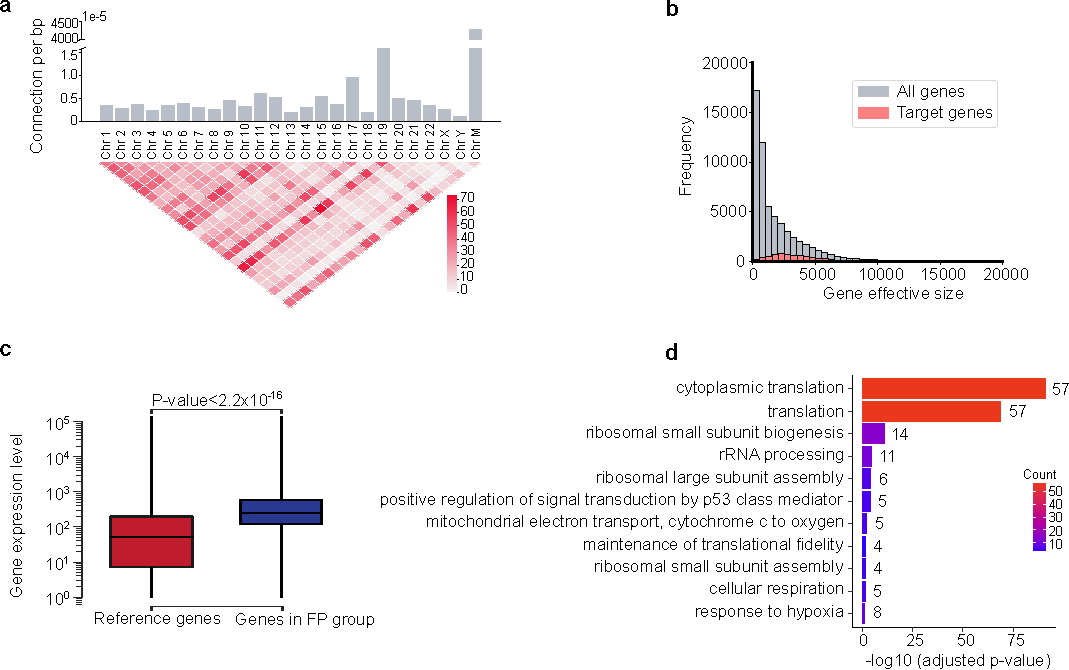
\includegraphics[height=1.2\columnwidth]{figures/finals/sf2}
     \caption{ {\bf  Analysis of \gls{fp} chimeric reads } (a) Visualization of chromosomal connections for all \gls{fp} chimeric reads detected in the VCaP 002 dataset. (b) Distribution of \gls{fp} biological processes enriched among \gls{fp} group genes in A549. (c) Distribution of \gls{fp} biological processes enriched among \gls{fp} group genes in HCT116. (d) Distribution of \gls{fp} biological processes enriched among \gls{fp} group genes in MCF7. (e) Distribution of \gls{fp} biological processes enriched among \gls{fp} group genes in K562. (f) Distribution of \gls{fp} biological processes enriched among \gls{fp} group genes in HepG2. (g) Distribution of \gls{fp} biological processes enriched among \gls{fp} group genes in VCaP.}
     \label{fig:sf2}
 \end{figure}


\newpage

\section{Supplementary information}

\renewcommand{\figurename}{Supplementary Fig.}
\renewcommand{\tablename}{Supplementary Table}


% If your article has accompanying supplementary file/s please state so here.
% Authors reporting data from electrophoretic gels and blots should supply the full unprocessed scans for key as part of their Supplementary information. This may be requested by the editorial team/s if it is missing.
% Please refer to Journal-level guidance for any specific requirements.


\begin{table}
	\centering
	\caption{Hyperparameter ranges used}
    \label{tab:nucleotideTRX_hyperparameter}
	\begin{tabular}{lc}
		\toprule
		                                    & {$\sf DeepChopper$}                  \\
		\midrule
		Layers                              & 2                                 \\
		Width                               & 256                               \\
		Parameters                          & 1.6M                              \\
		Optimizer                           & AdamW                             \\
		Optimizer momentum                  & $\beta_1$, $\beta_2$ = 0.9, 0.999 \\
		Training epoch                      & 100                               \\
		Batch size                          & 256-1024                          \\
		Learning rate                       & 2e-4 to 1e-3                      \\
		LR scheduler                        & Cosine decay                      \\
		Weight decay (model)                & 0-0.2                             \\
		Weight decay ({$\sf Hyena$} layers) & 0                                 \\
		Embed dropout                       & 0-0.2                             \\
		Residual dropout                    & 0-0.2                             \\
		Sequence lengths                    & 32769                             \\
		\midrule
	\end{tabular}

\end{table}


\begin{table}
    \caption{Open source libraries (and corresponding licenses) used in this work.}
    \label{tab:assets}
            \begin{tabular}{ll}
                \toprule
                Library                                                & License                                                                            \\ \midrule
                GenomicsBenchmark~\cite{grevsova2023genomic}           & Apache 2.0                                                                         \\
                Mamba~\cite{gu2023mamba}                               & Apache 2.0                                                                         \\
                HuggingFace~\cite{wolf2019huggingface}                 & Apache 2.0                                                                         \\
                Hydra~\cite{Yadan2019Hydra}                            & MIT                                                                                \\
                HyenaDNA~\cite{nguyen2024hyenadna}                     & Apache 2.0                                                                         \\
                NumPy~\cite{harris2020array}                           & \href{https://numpy.org/doc/stable/license.html}{NumPy license}                    \\
                Matplotlib~\cite{Hunter2007}                           & \href{https://matplotlib.org/stable/users/project/license.html}{Matplotib license} \\
                OmegaConf                                              & BSD 3-Clause                                                                       \\
                Pandas \cite{reback2020pandas}                         & BSD 3-Clause ``New" or ``Revised"                                                  \\
                PyTorch~\cite{paszke2019pytorch}                       & BSD-3 Clause                                                                       \\
                PyTorch Lightning~\cite{Falcon_PyTorch_Lightning_2019} & Apache 2.0                                                                         \\
                Seaborn~\cite{Waskom2021}                              & BSD 3-Clause ``New" or ``Revised"                                                  \\ \bottomrule
            \end{tabular}
\end{table}





% \section*{Declarations}

% Some journals require declarations to be submitted in a standardised format. Please check the Instructions for Authors of the journal to which you are submitting to see if you need to complete this section. If yes, your manuscript must contain the following sections under the heading `Declarations':
%
%\begin{itemize}
%	\item Funding
%	\item Conflict of interest/Competing interests (check journal-specific guidelines for which heading to use)
%	\item Ethics approval and consent to participate
%	\item Consent for publication
%	\item Data availability
%	\item Materials availability
%	\item Code availability
%	\item Author contribution
%\end{itemize}

%
%\begin{appendices}
%	\printglossary[type=\acronymtype, title=Abbreviations]
%
%	\section{Section title of first appendix}\label{secA1}
%
%	An appendix contains supplementary information that is not an essential part of the text itself but which may be helpful in providing a more comprehensive understanding of the research problem or it is information that is too cumbersome to be included in the body of the paper.
%
%	%%=============================================%%
%	%% For submissions to Nature Portfolio Journals%%
%	%% please use the heading ``Extended Data''.   %%
%	%%=============================================%%
%
%	%%=============================================================%%
%	%% Sample for another appendix section			               %%
%	%%=============================================================%%
%
%	%% \section{Example of another appendix section}\label{secA2}%
%	%% Appendices may be used for helpful, supporting or essential material that would otherwise
%	%% clutter, break up or be distracting to the text. Appendices can consist of sections, figures,
%	%% tables and equations etc.


%\end{appendices}

%%===========================================================================================%%
%% If you are submitting to one of the Nature Portfolio journals, using the eJP submission   %%
%% system, please include the references within the manuscript file itself. You may do this  %%
%% by copying the reference list from your .bbl file, paste it into the main manuscript .tex %%
%% file, and delete the associated \verb+\bibliography+ commands.                            %%
%%===========================================================================================%%


%% if required, the content of .bbl file can be included here once bbl is generated
%%\input sn-article.bbl

\end{document}
